Die Erste Regel des Mentoring ist: alle reden über das Mentoring.
Die Zweite Regel des Mentoring ist: ALLE reden ÜBER das Mentoring.
Die Mittlere Regel des Mentoring ist: wenn jemand schlappmacht... naja, dafür sind wir ja da.
Die Vorletze Regel des Mentoring ist: was im Mentoring gesagt wird, bleibt im Mentoring.
Die Letzte Regel des Mentoring ist: wer neu ist muss rein... ne, wirklich. Ist so.

Die Veranstaltung ''STO (STudienOrientierung) - Einführung in das Studium'', im Volkmund ''Das Mentoring'' genannt, ist Teil des sogenannten Ergänzungsmoduls und ihr \emph{müsst} es besuchen, um euren Bachelor Informatik zu bekommen. Ihr verdient hier sage und schreibe ganze \emph{2 CP}, wenn ihr es jetzt und sofort, also im \textbf{ersten Semester} besucht. \emph{Nur 1 CP} hingegen bekommt ihr, wenn ihr dieses Modul in einem späteren Semester abschließt. Überdies sind die Informationen, die ihr dort bekommt, vor allem in den ersten Semestern relevant. Weil STO überhaupt nicht anstrengend ist, könnt ihr es problemlos neben all den anderen Dingen besuchen, die euch möglicherweise viel Zeit und viele Nerven rauben. Außerdem soll euch genau jene Veranstaltung gerade ein kleines bisschen ein Führer durch den Informatik-Uni-Dschungel sein und dabei helfen, dass ihr vielleicht nicht ganz so viel Zeit und Nerven verliert. 

Was?: STO besteht aus einer Vorlesung und einem Kleingruppentreffen (mit 5 Terminen, über das Semester verteilt), genannt Peer-Mentoring. 

Warum?: Es geht hier darum, dass ihr den Einstieg in euer Studium besser findet, denn aller Anfang ist schwer. Im Laufe eures Studiums werdet ihr merken, dass an der Uni zu studieren auch bedeutet, eigenverantwortlich zu arbeiten: Ihr habt kaum Anwesenheitspflichten, müsst euch euren Stundenplan (zumindest später) selbst zusammenstellen und könnt selbst entscheiden, wie viel Übungs- und Lernaufwand ihr betreiben wollt. 
Ihr habt also viele Freiheiten, solltet dabei aber nicht den Kopf verlieren. Der Kopf bleibt auf dem Hals und ihr behaltet von dort aus den Überblick, wenn ihr möglichst viel über euer Studium wisst, denn dann könnt ihr anständig planen.
Die STO-Vorlesung und das Mentoring (Kleingruppentreffen) sollen euch dabei helfen, dieses Studienwissen zu erlangen. Alle Fragen die ihr rund um das (Informatik-)Studium habt, sollt ihr im Mentoring stellen. Ihr könnt dort außerdem thematisieren (oder euren Mentor direkt persönlich ansprechen), wenn sich euer Leben durch das Studium verändert hat und ihr an dieser Stelle Ratschläge braucht. Das bedeutet natürlich, dass alles was im Mentoring gesagt wird, auch im Mentoring bleiben soll.

Wie?: Ihr besucht die erste STO-Vorlesung am \textbf{16.04.2015} (Vorlesungsverzeichnis) und erfahrt dort, wie ihr euch in die Mentorings einschreibt.

 
\begin{center}
	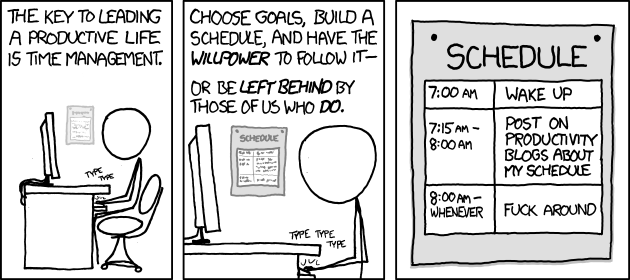
\includegraphics[scale=1.0]{comics/time_management.png}
\end{center}
